\documentclass[11pt]{article}

\usepackage{latexsym}
\usepackage{amsmath}
\usepackage{amssymb}
\usepackage{amsthm}
\usepackage{graphicx}
\usepackage{wrapfig}
\usepackage{pseudocode}
\usepackage{url}
\usepackage[backref, colorlinks=true, citecolor=red, urlcolor=blue, pdfauthor={Jyh-Ming Lien}]{hyperref}


\newcommand{\handout}[5]{
  \noindent
  \begin{center}
  \framebox{
    \vbox{
      \hbox to 5.78in { {\bf } \hfill #2 }
      \vspace{4mm}
      \hbox to 5.78in { {\Large \hfill #5  \hfill} }
      \vspace{2mm}
      \hbox to 5.78in { {\em #3 \hfill #4} }
    }
  }
  \end{center}
  \vspace*{4mm}
}

\newcommand{\lecture}[4]{\handout{#1}{#2}{#3}{#4}{#1}}

\newtheorem{theorem}{Theorem}
\newtheorem{corollary}[theorem]{Corollary}
\newtheorem{lemma}[theorem]{Lemma}
\newtheorem{observation}[theorem]{Observation}
\newtheorem{proposition}[theorem]{Proposition}
\newtheorem{definition}[theorem]{Definition}
\newtheorem{claim}[theorem]{Claim}
\newtheorem{fact}[theorem]{Fact}
\newtheorem{assumption}[theorem]{Assumption}

% 1-inch margins, from fullpage.sty by H.Partl, Version 2, Dec. 15, 1988.
\topmargin 0pt
\advance \topmargin by -\headheight
\advance \topmargin by -\headsep
\textheight 8.9in
\oddsidemargin 0pt
\evensidemargin \oddsidemargin
\marginparwidth 0.5in
\textwidth 6.5in

\parindent 0in
\parskip 1.5ex
%\renewcommand{\baselinestretch}{1.25}
\graphicspath{ {images/} }

\begin{document}

\lecture{Programming Assignment 2 report}{Fall 2017}{Faez Dabestani Ziabari}{Computational Geometry}

\section{Summary of the two methods}

\subsection{hedcuter method}
Abstract: The hedcuter algorithm generates a number of points (this number can be given by the user) with a bias towards the darker areas; then treating these points as Voronoi sites, creates a Voronoi graph (either with or with out the GPU) and tessellates the image. Then, using a density function, the method needs to find the weighted center of each cell and replace that point as the new site of the cell. The algorithm then Recomputes the Voronoi graph, moving the center each time, over and over until the new weighted centers stay the same as the old ones (with in a margin of error), or until the code runs out of a certain predetermined number of iterations.

In the following paragraphs, I will recount some  the key details of this implementation. First off, the way hedcuter initializes the given number of random points with a bias towards darker areas, is by getting random points repeatedly, and discarding them with a probability. If the generated point is a repeat (has already been visited), we discard the point immediately. Otherwise, the point is discarded randomly with a weighted probability, increasing the likelihood of discarding a point if it is brighter. This is to reduce the number of iterations, and start the process off in an approximation of the final image. 

To define a Voronoi cell, the program uses a structure that holds the \underline{site} of the cell, and a list of \underline{every single point} in that cell. The creation of the Voronoi diagram can be done using or not using the GPU. When using the GPU, the graph is discretely approximated using the cones generating method that we covered in class, then find the density center of each cell and relocating it. If the user decides against using the GPU, the method generates a Voronoi diagram, considering the color intensities of each pixel while doing so. First stipples are added to a vector, paired up with their color intensity, then the vector is sorted into a priority queue (which is very time consuming), and then propagates every pixel, spreading from every site to it's neighbors, to find out which site each pixel belongs to. 

Finally, the method moves the sites of each cell by computing the centroid of each cell. To find that point, we find the weighted average of the color intensities of every pixel in each cell. The whole process of the hedcuter method is terminated either based on the average displacement of the center of each cell, or just the maximum displacement. Depending on user input, when one of these desired numbers is optimally small, the stipples are considered converged. and the process is over.

\subsection{voronoi method}

Abstract: first create an initial distribution of stipples, again with bias towards darker regions, then find the Voronoi diagram treating the stipples as sites of the diagram, then finding the center of each cell using a density function, and moving each stipple to that center, repeating these steps until the stipples converge to the center of each cell permanently.

Similar to the first method, the first step is to generate n points, with biased towards the darker regions of the picture. The only difference of this method compared to the first method, is that this algorithm uses the generator function from Boost to generate a random point and randomly discard that point. Similar to the hedcut algorithm, It is much more likely for a point to get discarded, if the point is chosen from the lighter parts of the picture. 

Generating the Voronoi diagram in this method is very straight forward, using the Fortune's algorithm (or plain sweep) to find the cells. The fundamental difference being that in this method, we define each Voronoi cell as by the \underline{site} and the \underline{edges of the cell}. After that, same as the last method, we add all the pixels falling with in the bounds of a group of edges, to be considered inside of the correctly corresponding cell.

 Calculating the new centroid of each cell in this algorithm is much more complex. Using a function called 'create clipLine', the algorithm finds all the line formulas of the edges of each cell. Then, finding an imaginary bounding box for each cell, we select a number of points (Based on the default of inputted subpixel number), and only consider these points with of the cells. We approximate the intensity of the cell based on the intensity of these points (as opposed to what we did in the previous method where we calculated the intensity of every pixel), and find the average of those pixels to be the new centroid of the cell. 


\newpage\section{Comparison of the two methods}
On average, the hedcut method has a clear disadvantage on speed. Since there is no definite number of iterations before the distance converges to smaller numbers, the calculations can continue for random amounts of time. Yet, there is little competition in terms of which methods would finish first. Since I am a Windows user, I was forced to compile the code on a virtual Linux Ubuntu machine; which made the running time even longer. So I excuse my self from measuring actual time. 

We will answer multiple questions regarding the quality of these algorithms, but first lets have a side by side view of some of the outputs of these methods:
\newline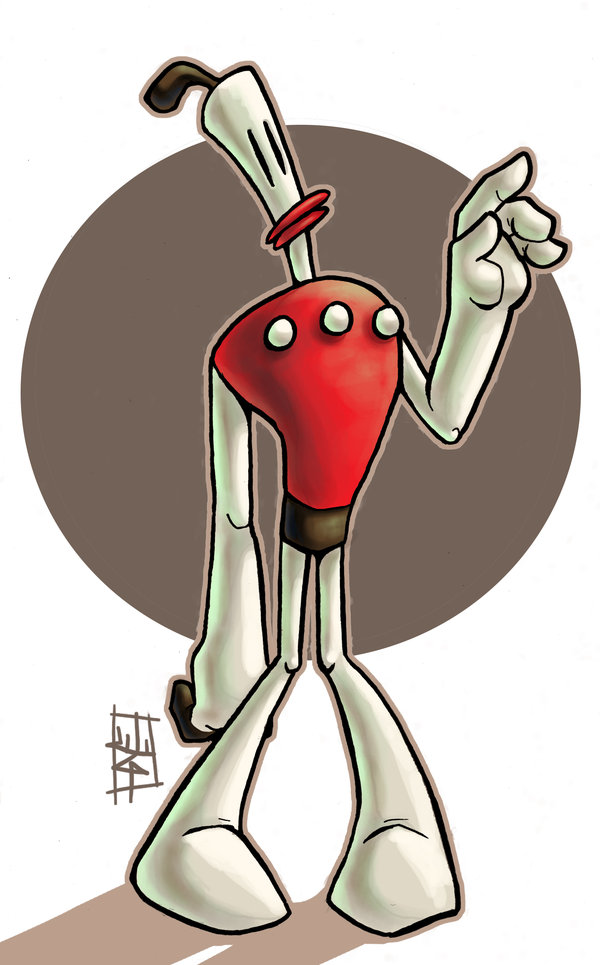
\includegraphics[width=5cm, height=8cm]{klaymen.png} 
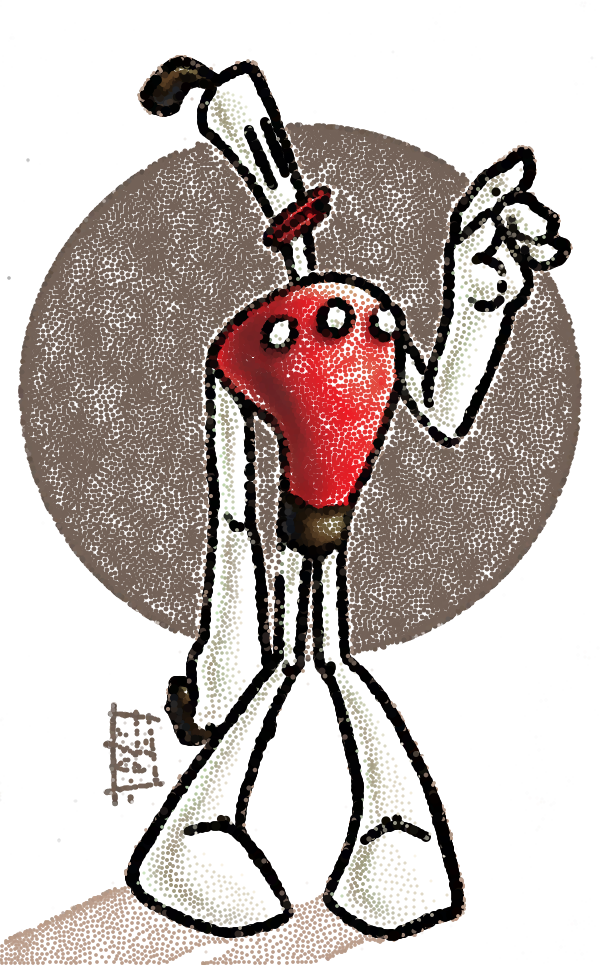
\includegraphics[width=5cm, height=8cm]{klaymen-hedcut-20000.png}
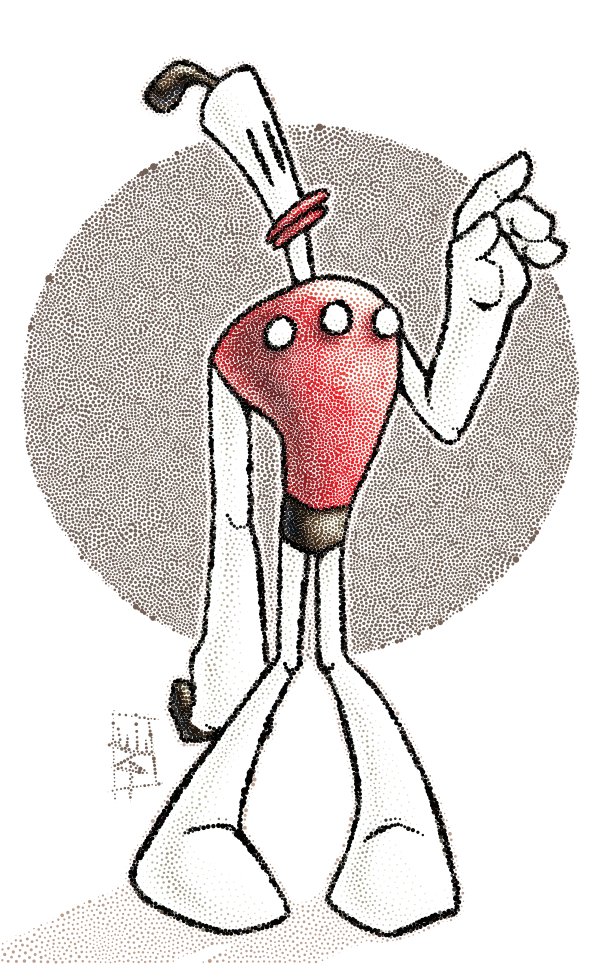
\includegraphics[width=5cm, height=8cm]{klaymen-voronoi-20000.png}
\newline Image 1: Klaymen from left to right Original - Hedcut - Voronoi 20,000 stipples 
\newline 
\newline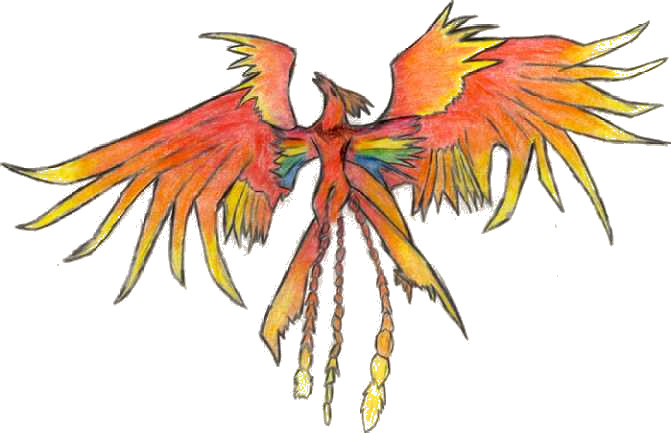
\includegraphics[width=5cm, height=4cm]{phoenix.png} 
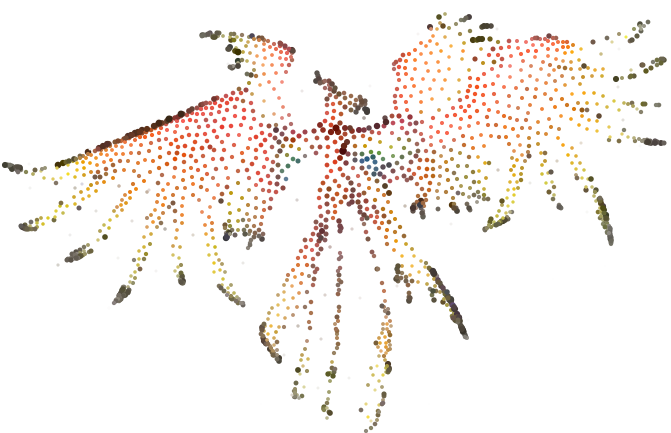
\includegraphics[width=5cm, height=4cm]{phoenix-hedcut-2000.png}
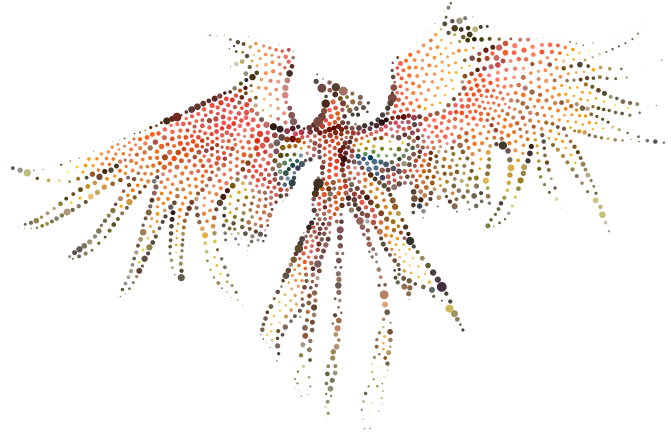
\includegraphics[width=5cm, height=4cm]{phoenix-voronoi-2000.png}
\newline Image 2: Phoenix from left to right Original - Hedcut - Voronoi 2,000 stipples
\newline
\newline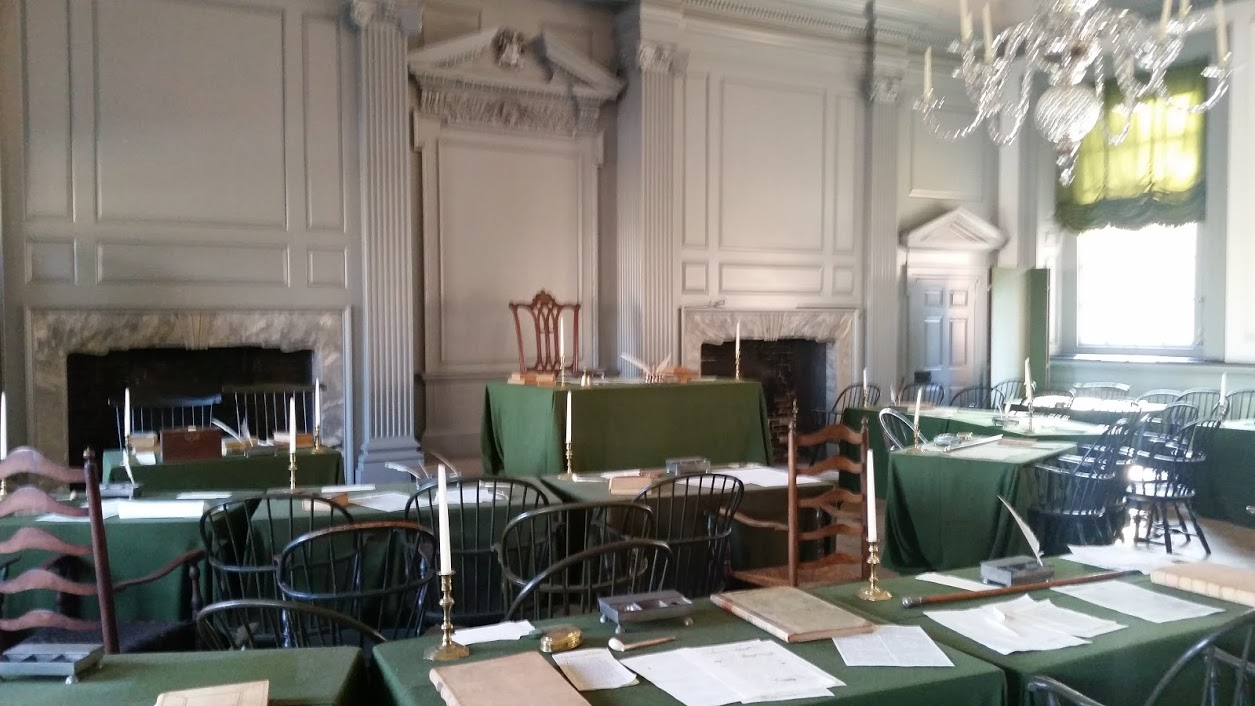
\includegraphics[width=6cm, height=5cm]{libertyhall.png} 
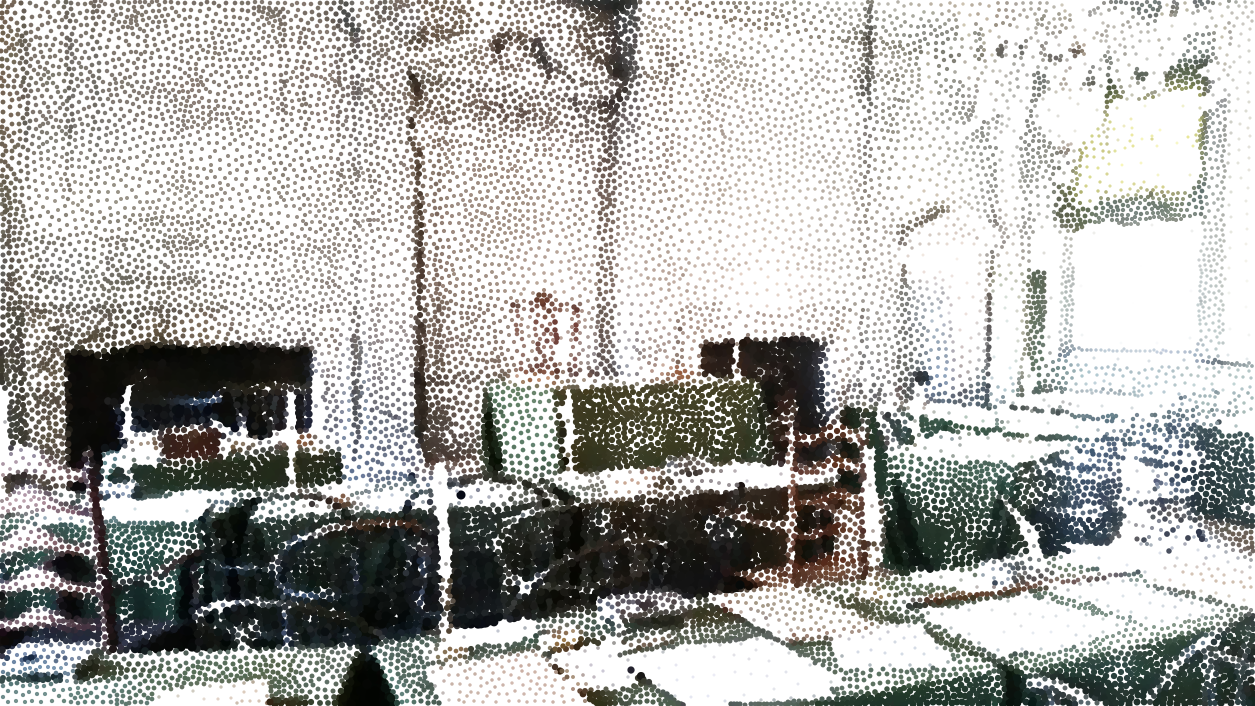
\includegraphics[width=6cm, height=5cm]{libertyhall-hedcut-20000.png}
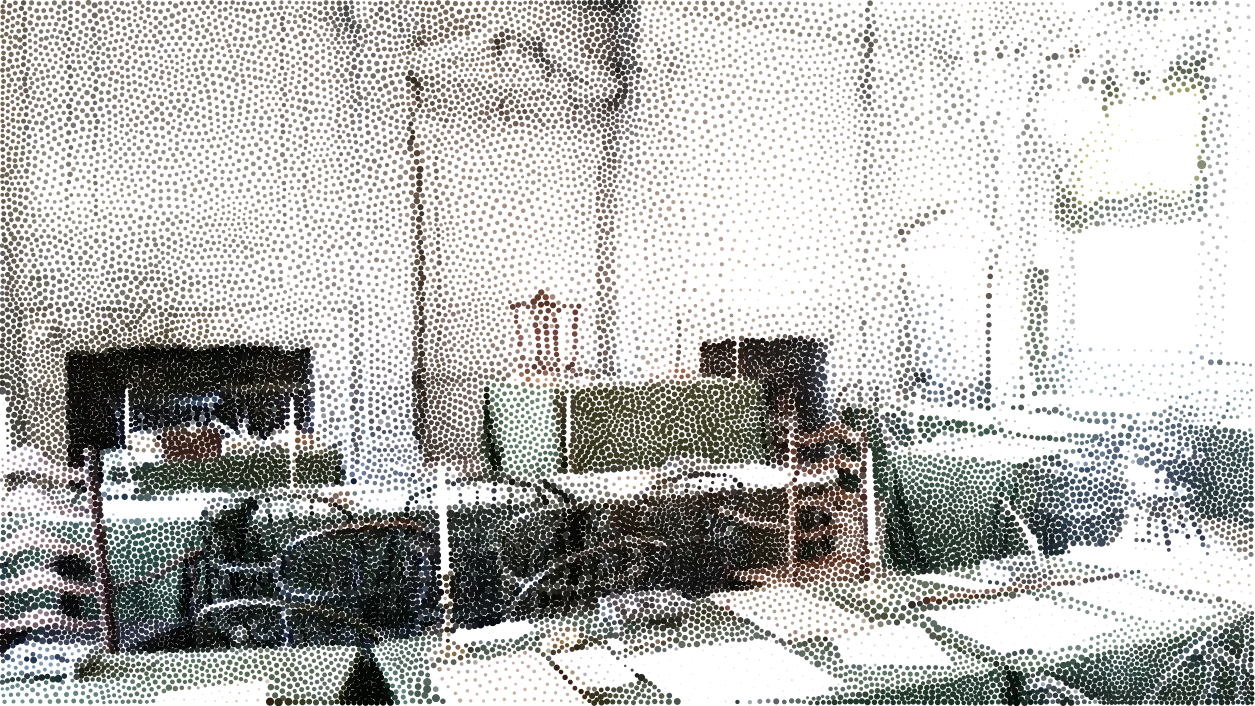
\includegraphics[width=6cm, height=5cm]{libertyhall-voronoi-20000.png}
\newline Image 3: Liberty hall from left to right Original - Hedcut - Voronoi 20,000 stipples
\newline 
\newline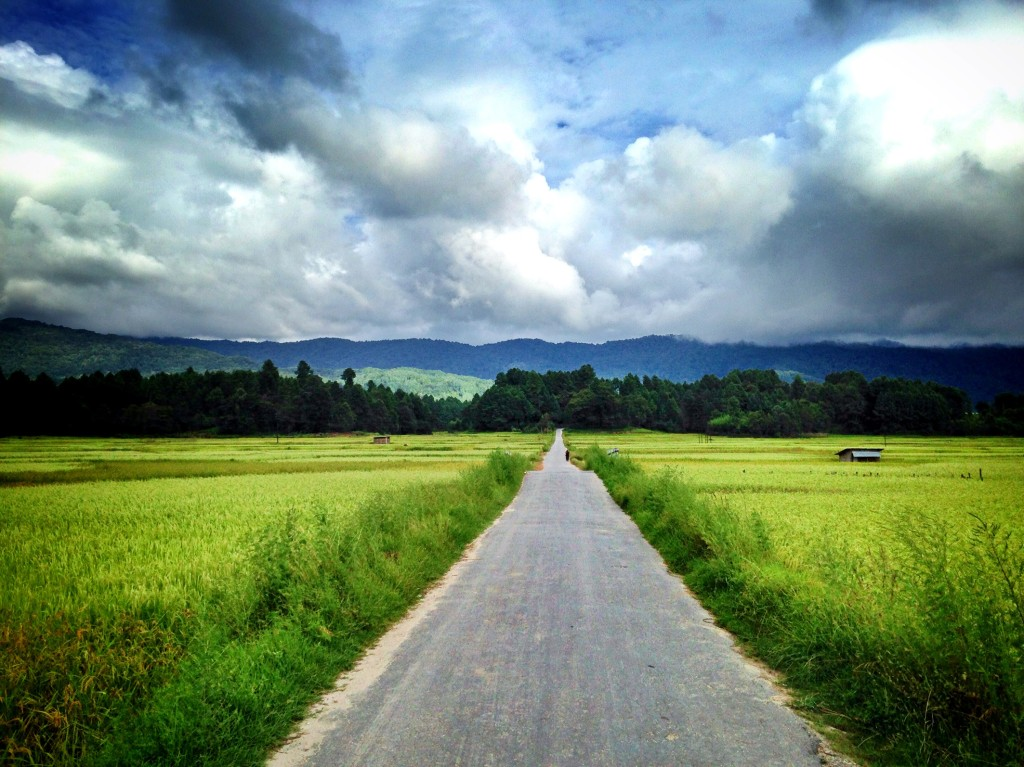
\includegraphics[width=6cm, height=5cm]{landscape.png} 
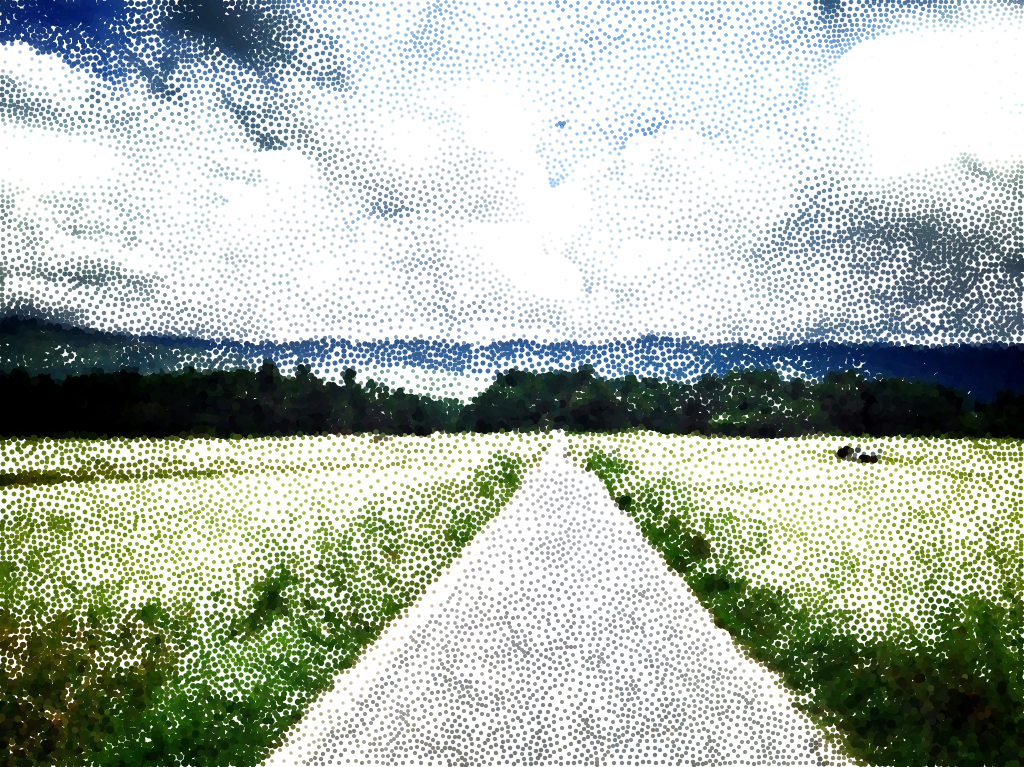
\includegraphics[width=6cm, height=5cm]{landscape-hedcut-20000.png}
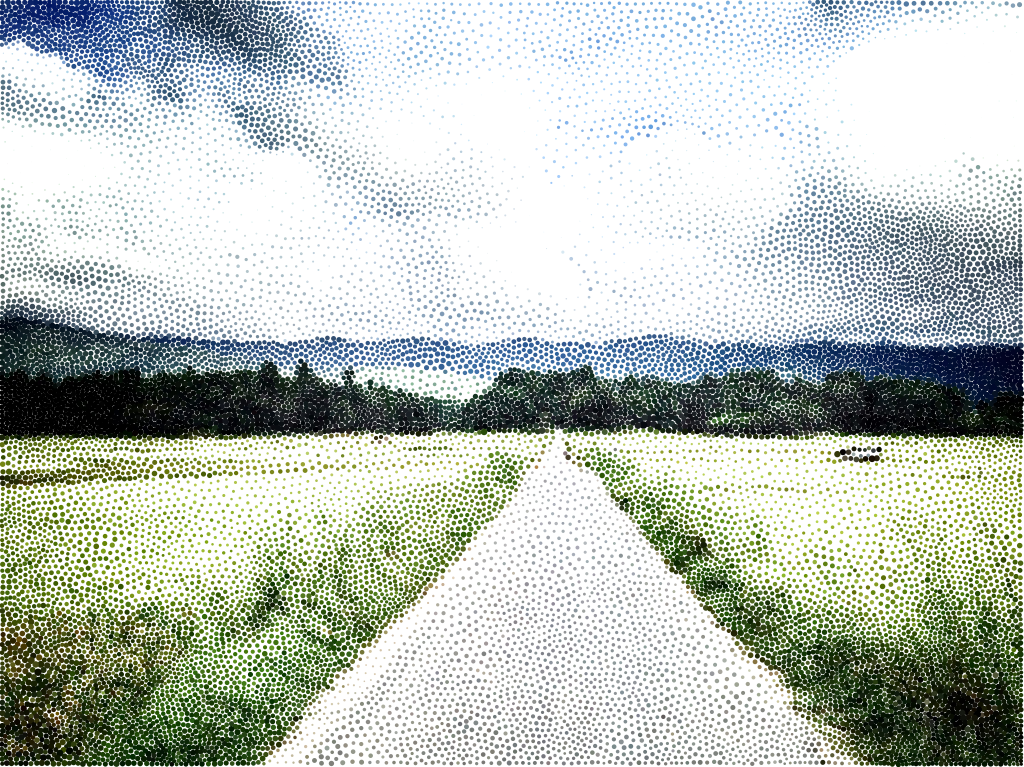
\includegraphics[width=6cm, height=5cm]{landscape-voronoi-20000.png}
\newline Image 4: Random landscape from left to right Original - Hedcut - Voronoi 20,000 stipples
\newline 
\newline
\includegraphics[width=6cm, height=4.5cm]{sanders.png} 
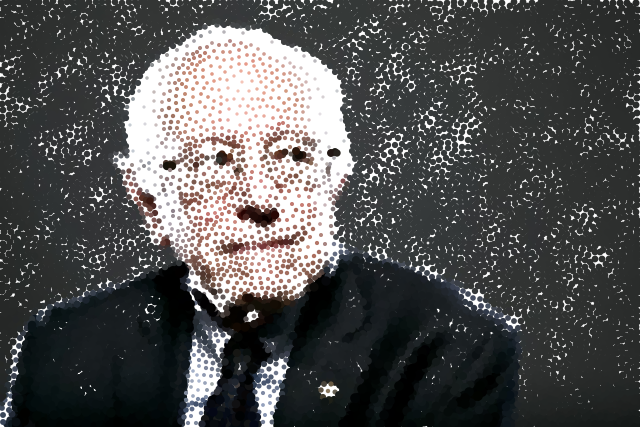
\includegraphics[width=6cm, height=4.5cm]{sanders-hedcut-10000.png}
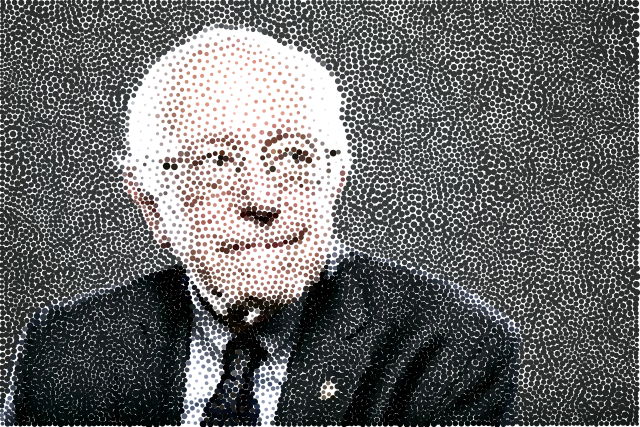
\includegraphics[width=6cm, height=4.5cm]{sanders_voronoi_10000.png}
\newline Image 5: Bernie Sanders from left to right Original - Hedcut - Voronoi 10,000 stipples

\textbf{Question 1.} Do you get the same results by running the same program on the same image multiple times?

\textbf{Answer:} No. Every time the images look slightly different. This is due to the randomized nature of the initial stipple points. 

\textbf{Question 2.} If you vary the number of the disks in the output images, do these implementations produce the same distribution in the final image? If not, why?

\textbf{Answer:} Well points always gravitate towards darker areas. So the image never looks completely different or the same  given different number of disks. The Voronoi method actually by default adapts, by changing the size of these disks to fill out more area. Which makes the images more similar to the images of the print outlets publishing hedcuts. 

\textbf{Question 3.} If you vary the number of the disks in the output images, is a method faster than the other?

\textbf{Answer:} This depends on how much we reduce the number of disks in comparison to the other method. As mentioned, the second method usually concludes much faster than the first method. So to reduce the number of stipples on the first method to the point that it becomes faster than the second method, would also reduce the quality of the outputted image to the point where it is basically unrecognizable. So technically yes... it just would look like a few points on a blank page.

\textbf{Question 4.} Does the size (number of pixels), image brightness or contrast of image increase or decrease their difference?

\textbf{Answer:} The size does not, because you need to find the magic number of disks that covers all of the screen anyways. But the brightness does make a fairly important difference. An image with a dark background yields results surprisingly faster using the first algorithm (Faster than it does on a brighter image, but still not as fast as the second algorithm). In this example, image 5 converged in 28 iterations on hedcut, where image 2 did not converge until it ran out of maximum iterations. So unless the code has a political bias hard coded, I think the darker the image, the faster the hedcut code converges. 

\textbf{Question 5.} Does the type of image (human vs. machine, natural vs. urban landscapes, photo vs. painting,etc) increase or decrease their difference?

\textbf{Answer:} As can be seen, I have made an attempt to address this question with my choice of output images. Though I honestly doubt that the humanity of the subject of a picture is going to make any kind of a significant impact, I have images that illustrate the difference in quality between drawn vs. photographed, indoor vs. outdoor, single subject vs. multiple objects, and predominantly light vs predominantly dark. As was mentioned before, the darker the image, the faster the computation time for the hedcut and even Voronoi. The scenery images seem to perform worse than single subject images, due to the variations of the colors (contrasts), and the usual mandate of them to be lighter overall. 

As can be seen, in all of these cases, with the same amount of stipple points, we more often than not get better results with the Voronoi method. The dynamic sizing of the disks seems to suggest a higher level of sophistication, which allows the user to not need to struggle to find the best number of stipples, regardless of the type and size of the image. 

\textbf{Question 6.} Are the outputs of these stippling methods different from the hedcut images created by artists (e.g.those from the Wall Street Journal)?

\textbf{Answer:} To address this question it is only fair to consider the single subject images, and not the scenery. And even then... I would say no. Neither of these methods perform as well as a real artist. Mostly, because an artist makes good design decisions, deciding whether to include some background elements or not, and to emphasize certain parts of the picture more, even though they are not in reality darker than the others. The first method is particularly bad at this, since when too many points are used, the image completely breaks the structure of standalone points, turns into patches of connected sections. 

Again the fact that the Voronoi method dynamically sizes the points by default comes at a major advantage here, and makes these images look like the real inspirations for the hedcut artist. The images output by the second algorithm, look like actual old timely printed images, rather than an artists imitation of those prints. 

\section{Improvement of hedcuter method}

\textbf{Improvement 1}- Better Initial Stippling: 

As was mentioned in "Weighted Voronoi stippling" paper, if we start out with a better approximation of the final answer, the faster will we conclude our stippling process. Which is why in both methods there are mechanisms to initialize the stipples with a major bias towards darker regions of the images.

However, when the hedcut method runs in debug mode, it is immediately obvious that this is hardly the case, since the initial distribution still is allowing for too many points to be picked out of the lighter parts of the images, as you can see from this screen grab:
\newline

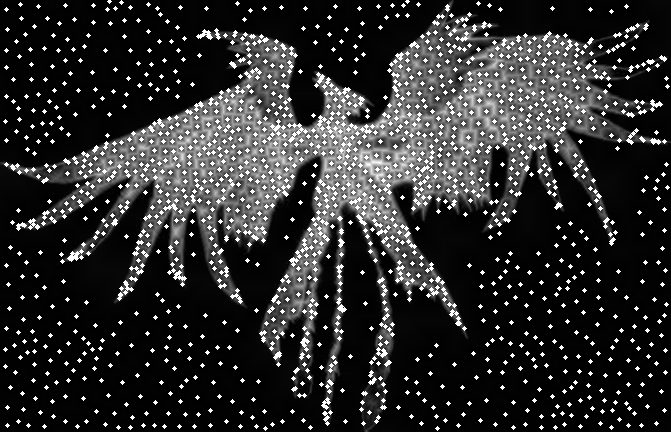
\includegraphics[width=12cm, height=8cm]{Pheonix-Debug-Normal.png} 
\newline Image 6: Phoenix using 2,000 stipples, no changes

As can be seen, even though the points are much more likely to be in the colored areas, there are still way too many points in the blank areas of the picture. It is in our interest to reduce this likely hood as much as possible. The hedcuter code uses a Gaussian distribution to bias the points being picked. I had the idea to use an exponential distribution to bias the points in favor of being chosen from the darker sides. That way, the lighter points are still likely to be chosen, but the lighter the points, the exponentially less likely they would be to be picked as a stipple point. 

So as my first improvement, I have re-written the "sample\_initial\_points" function to bias the stippling with exponential likely hoods. The "std::exponential\_distribution" function demands a standard deviation, and experimenting with that, I found the best number to be 7 (which is the default of my code now). But I have also allowed the user to be able to pick this number.

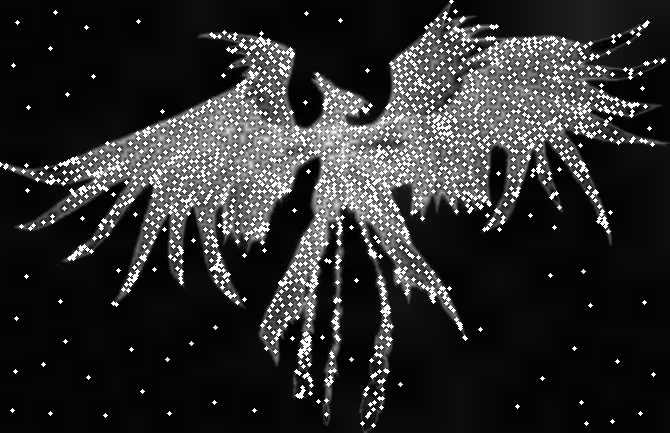
\includegraphics[width=12cm, height=8cm]{3point5Phoenix.png} 
\newline Image 7: Phoenix using 2,000 stipples, exponential distribution at 3.5

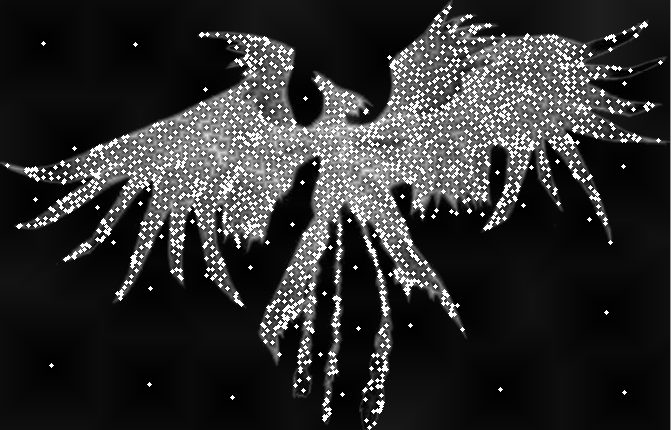
\includegraphics[width=12cm, height=8cm]{5Phoenix.png} 
\newline Image 7: Phoenix using 2,000 stipples, exponential distribution at 5 


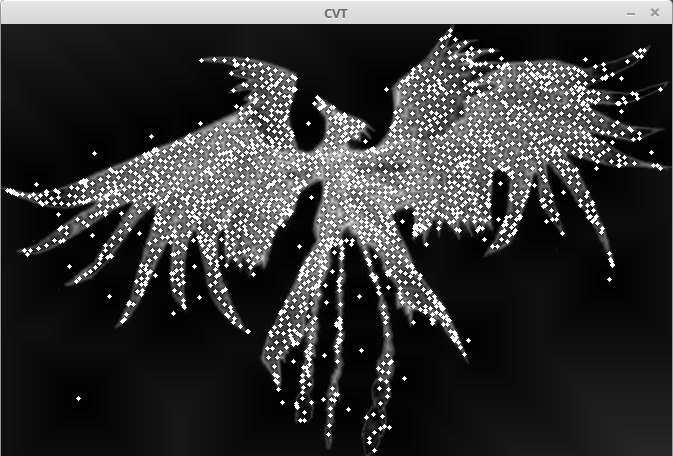
\includegraphics[width=12cm, height=8cm]{7phoenix.png} 
\newline Image 7: Phoenix using 2,000 stipples, exponential distribution at 7 

As can be seen, this method proved to be very effective. This reduces the computation time reasonably, since the initial estimation is already close to the final image. As was mentioned, I have made it so the user can change this deviation variable by typing -deviation followed by a floating point number in the command line while running the code. Though \underline{the number must be smaller than 10, and using a larger number will case the program to fall in an infinite loop.}

\textbf{Improvement 2}- Dynamic sizing and Collision avoidance: (Feel free to count this as 2 improvements!)

A fairly big advantage of the Voronoi method, was the fact that it could dynamically decide the size of every Voronoi cell. The way that method was able to do this, was by finding the distance of the centroid from each edge of the cell, and picking the longest or the shortest distance depending if overlapping was allowed or not. In the hedcut method, our data structure does not hold the edges of each cell, so we need to find another way of deciding the radius of the disks. 

To find the actual edges of each cell, we would need a convex haul, which would take O(n.log(n)) time. We would use plain sweep, and find the edge, and be able to find each of the radiuses. Even though that is an efficient strategy, this algorithm already takes far too long to compute, and we already have a lot of memory occupied. So I came up with an O(n) time algorithm to give an educated guess as to what the radius of the cell should be. 

So, in my improvement, I sweep over the coverage list (the list of all the pixels in a cell), and find the points on the edges directly to the top, bottom, left and right of the centroid. Using these points we have 2 guesses as to what the radius can be, which are the distance of the points across from each other. The larger of these points can be for when we don't mind collisions, and the smaller one, for when we do want to avoid collisions. 

Now I am under no illusions; this method is not guaranteed or optimal. It is very much possible to pick the smallest of these distances and still end up colliding with other cells. But it is an educated guess, with less time spent trying to find. As with the last improvement, I have added a command "-noCollisions", that would allow the user to control which one of these radiuses should be used.

Here are a couple of new outputs. To underscore the helpfulness of these changes, I am comparing 2 images that would have been done terribly if it hadn't been for dynamic sizing. Before the dynamic size, I made the disk size of these images too small. Observe how the dynamic sizing overrides the disk size, when the uniform-disk-size variable is false, to give a better approximation of the images: 

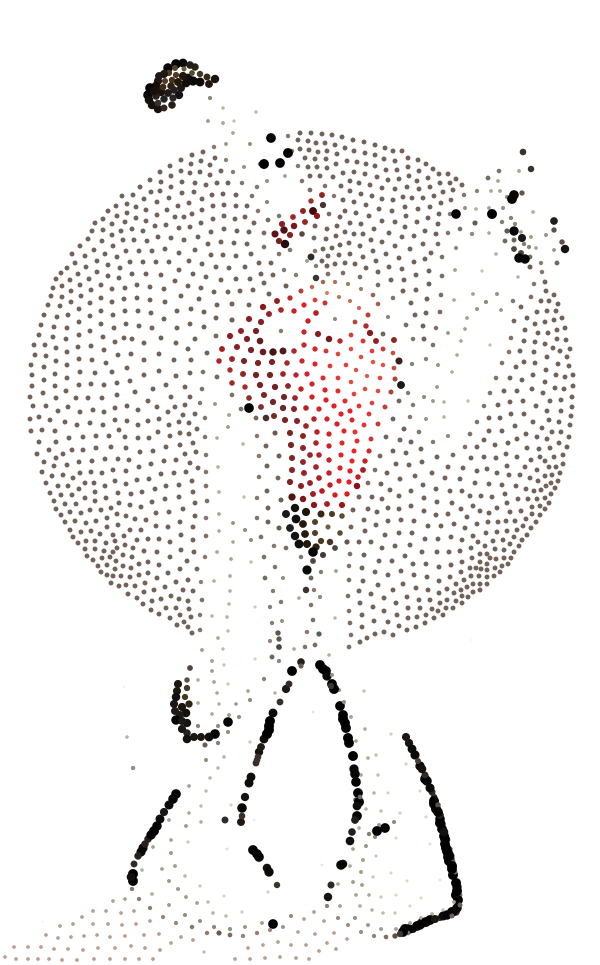
\includegraphics[width=5cm, height=8cm]{klaymen-old-2000.png} 
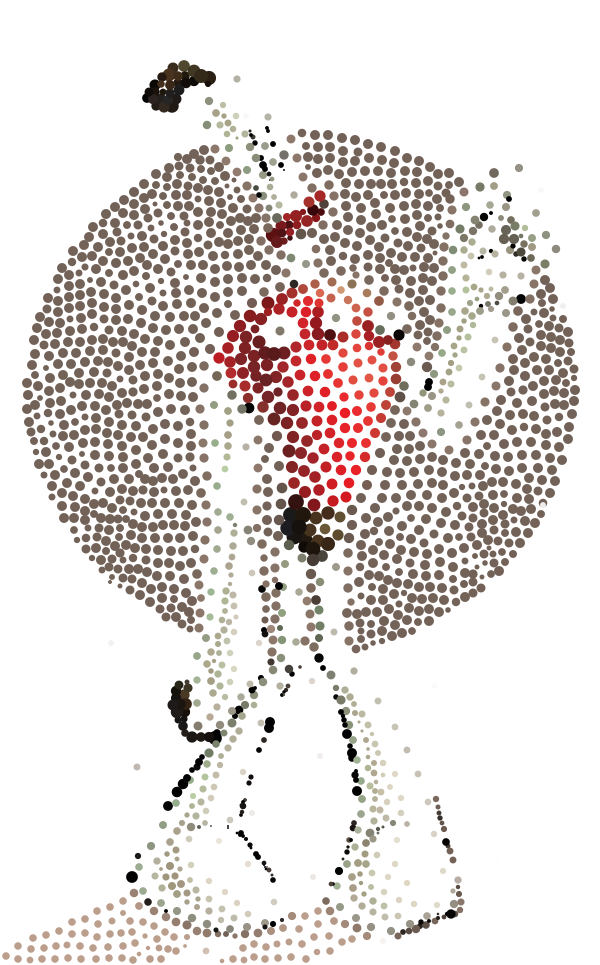
\includegraphics[width=5cm, height=8cm]{klaymen-new-2000.png}
\newline Image 8: Klaymen statically, vs Dynamically sized, with 2000 stipples 


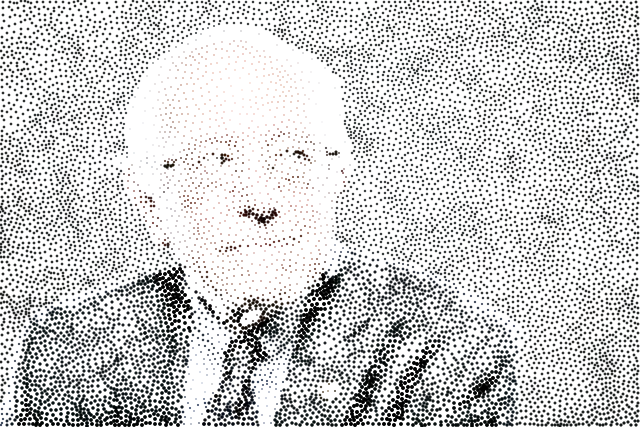
\includegraphics[width=8cm, height=6.5cm]{sanders-old-10000.png} 
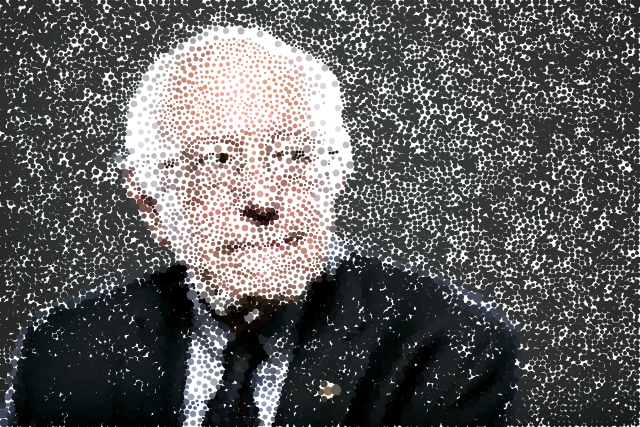
\includegraphics[width=8cm, height=6.5cm]{sanders-new-10000.png}
\newline Image 9: Bernie Sanders statically, vs Dynamically sized, with 10000 stipples 

This improvement still does not give results as good as the Voronoi method, but the results after this improvement look more similar to the Voronoi method than they used to. 



\bibliographystyle{plain}
\bibliography{report}

\end{document}


